\documentclass[border=0.8ex,svgnames,tikz]{standalone}
\usepackage{amsmath,mathtools}
\usepackage{fontspec}
\setmainfont{Source Serif 4}
\setsansfont{Source Sans 3}
\setmonofont{Source Code Pro}
\usepackage{ifthen}
\usetikzlibrary{chains,shapes.multipart}
\newcommand\mystrut{\vrule height 0.85em depth 0.25em width 0pt}
\begin{document}
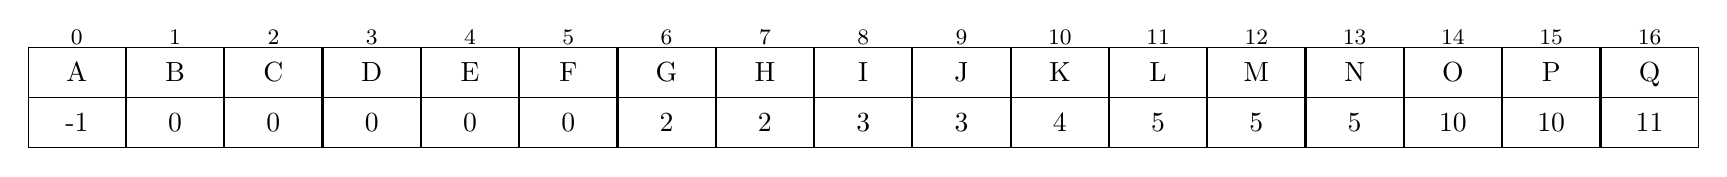
\begin{tikzpicture}[node distance=0,start chain=going right]
  \begin{scope}[
    every node/.style={
      draw,
      on chain,
      align=center,
      text width=1cm,
      rectangle split,
      rectangle split parts=2,
    },
    ]
    \foreach[count=\i from 0] \val/\parent in
    {A/-1,B/0,C/0,D/0,E/0,F/0,G/2,H/2,I/3,J/3,K/4,L/5,M/5,N/5,O/10,P/10,Q/11}
    {
      \node(node\i){
        \nodepart{one}\mystrut\val
        \nodepart{two}\mystrut\parent
      };
    }
  \end{scope}
  \begin{scope}[
    every node/.style={
      draw=none,
      align=center,
      font=\footnotesize,
      inner sep=0.2ex,
    },
    ]
    \foreach \i in {0,...,16}
    {
      \node[above=of node\i]{\i};
    }
  \end{scope}
\end{tikzpicture}
\end{document}
